\documentclass[catalan,border=15pt,class=scrartcl,multi=minipage,parskip=half*]{standalone}

% encoding
\usepackage[utf8]{inputenc}
\usepackage[T1]{fontenc}
\usepackage{lmodern}
\usepackage{babel}

% formatting and fixes
\frenchspacing
\usepackage[style=spanish]{csquotes}
\MakeAutoQuote{«}{»}
\usepackage{bookmark}

% ADD ANY SPECIFIC PACKAGES HERE
% (CHEMISTRY, CODE, PUBLISHING)
\usepackage[usenames,dvipsnames,svgnames,table]{xcolor}
\usepackage{adjustbox}
\usepackage{booktabs}
\usepackage{mathtools}
\usepackage{commath}
\usepackage{tikz}
\usepackage{siunitx}
\usepackage{nicefrac}
\usetikzlibrary{calc}
\usetikzlibrary{arrows.meta}
\usetikzlibrary{automata}
\usepackage{minted}

% other options
\setcounter{tocdepth}{6}
\setcounter{secnumdepth}{2}

% hyperlink setup / metadata
\usepackage{hyperref}
\AfterPreamble{\hypersetup{
  pdfauthor={Xavier Mendez},
  pdfsubject={IPAV},
  pdfpagelayout=OneColumn,
}}

% custom commands
\newcommand{\startpage}{\begin{minipage}{30em} \setlength{\parskip}{0.5em}}
\newcommand{\finishpage}{\end{minipage}}
\newcommand{\iopair}[2]{\( \left(#1\right) \rightarrow #2 \)}

\AfterPreamble{\hypersetup{
  pdftitle={Entregable 1: La señal de voz},
}}

\newcommand{\nodenamebit}[1]{\textsf{#1}}
\newcommand{\nodenamesingle}[2]{\textsf{#1}_\textsf{#2}}
\newcommand{\nodenamerange}[3]{\textsf{#1}_\textsf{#2..#3}}
%\newcommand{\nodenamesingle}[2]{\textsf{#1[#2]}}
%\newcommand{\nodenamerange}[3]{\textsf{#1[#2..#3]}}

\begin{document}
\startpage

\paragraph{Problema 1.} \hspace{1em}

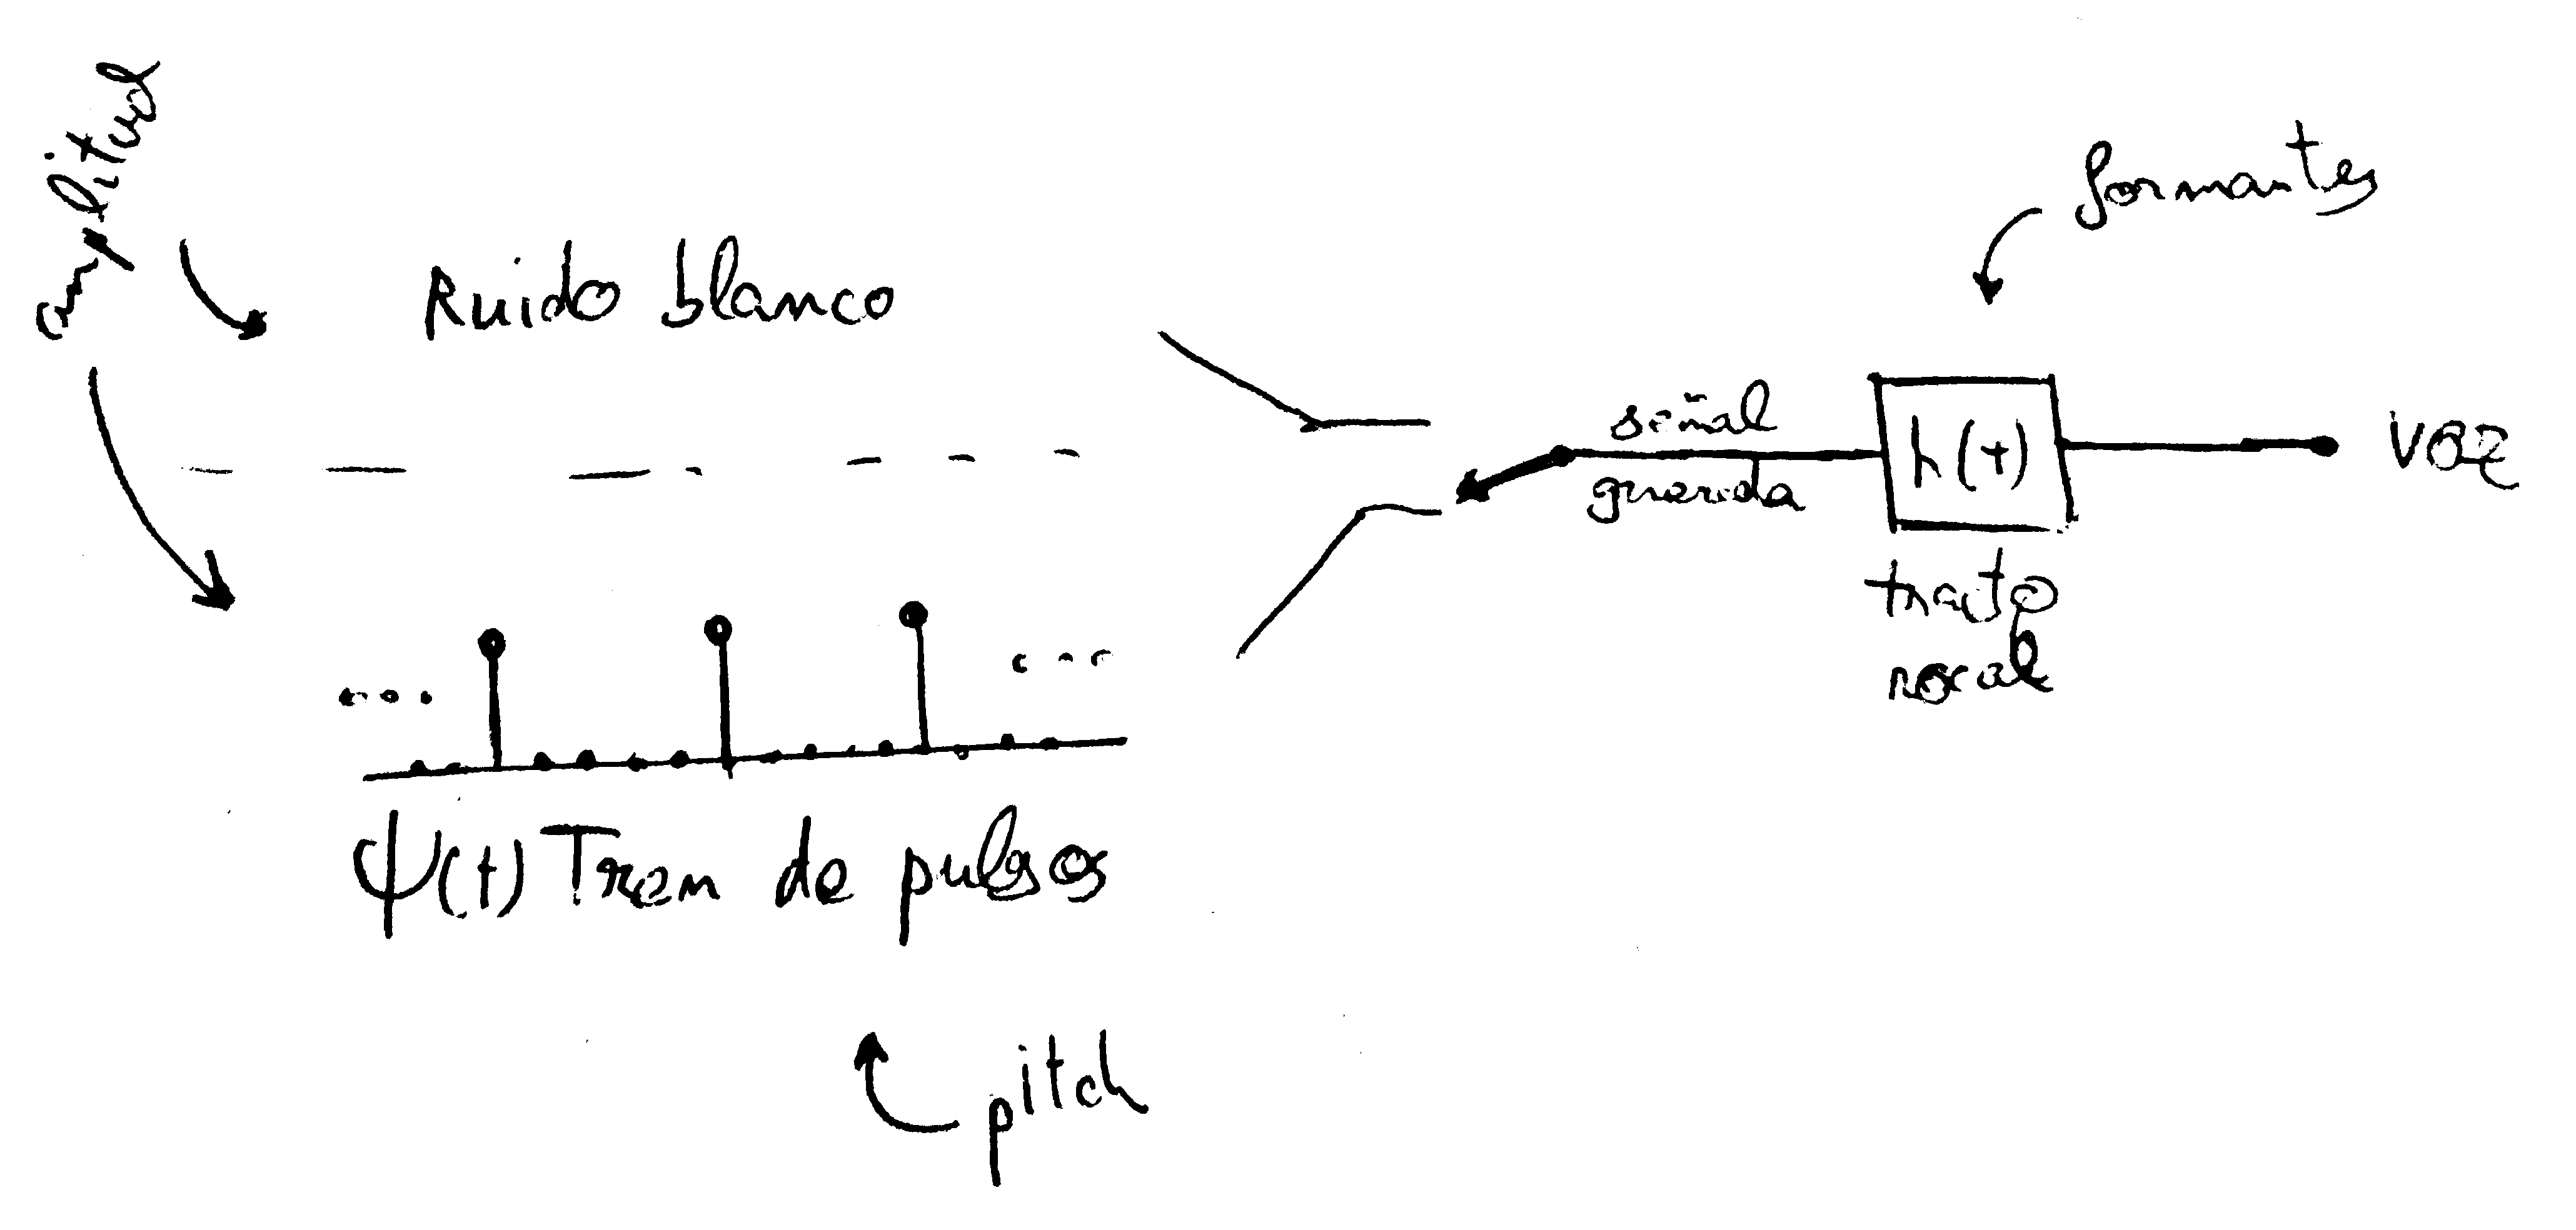
\includegraphics[width=\textwidth]{T1-p1}

\finishpage


\startpage
\paragraph{Problema 2.}

Los formantes son dos frecuencias a las que el tracto vocal ofrece una ganancia
especialmente alta. Se situan entre los \SI{200}{\hertz} y los \SI{2}{\kilo\hertz}
y su combinación determina el tipo de fonema que se percibe.

Si representamos la combinación de los dos formantes en un plano, y anotamos
las posiciones de las vocales, veremos que tienen una disposición similar a un
triángulo. Esto se llama \emph{triángulo vocálico} y sucede en el español y en
la mayoría de idiomas, si bien la forma puede ser algo
distinta.

\finishpage


\startpage
\paragraph{Problema 3.}

Los bins de la DFT correspondientes a las formantes son $n_1 \simeq 62$ y
$n_2 \simeq 135$. Segun $f = \nicefrac{n}{N} \, f_s$ con $f_s =
\SI{8}{\kilo\hertz}$ y $N = \num{1000}$, tenemos que los dos formantes son:
%
\begin{align*}
  f_1 \simeq \SI{496}{\hertz}
\\
  f_2 \simeq \SI{1080}{\hertz}
\end{align*}
%
Según la figura~2, esto corresponde a una vocal «o».

\finishpage


\startpage
\paragraph{Problema 4.}

\subparagraph{Apartado A.}

Respecto al pitch, la distancia entre los «deltas» (harmónicos) que se obserban
en la DFT es de unos \num{41} bins y por tanto \SI{200}{\hertz} sería la
frecuencia fundamental.

\subparagraph{Apartado B.}

Siguiendo el mismo procedimiento que en el problema~2, la envolvente alcanza
valores altos en aproximadamente $n_1 \simeq \num{110}; n_2 \simeq \num{360}$
que corresponden a las frecuencias $f_1 \simeq \SI{537}{\hertz}; f_2 \simeq
\SI{1758}{\hertz}$.

\subparagraph{Apartado C.}

En base a los dos formantes, la vocal parece ser una «e». La distancia es más
grande de lo habitual.

\finishpage


\startpage
\paragraph{Problema 5.}

\subparagraph{Apartado A.}

Sí, porque podemos apreciar múltiples sincs (armónicos) y separarlas con
suficiente claridad.

\subparagraph{Apartado B.}

Si la vocal es una «u», los formantes deben ser aproximadamente \SI{380}{\hertz}
y \SI{900}{\hertz}, y dado que $N = 500$ y corresponden a los bins \num{18} y
\num{63}, la frecuencia de muestreo que más cuadra es \SI{8}{\kilo\hertz}.

\subparagraph{Apartado C.}

La frecuencia fundamental es de 9 bins y por tanto \SI{144}{\hertz}.
Es muy arriesgado decir si corresponde a un hombre o a una mujer, aunque
es ligeramente más probable lo primero.

\finishpage


\startpage
\paragraph{Problema 6.}

\subparagraph{Apartado A.}

La frecuencia fundamental \SI{100}{\hertz} se situa en el bin \num{206}, y
$N = 2048$, con lo cual aislamos $f_s$ de $f = \nicefrac{n}{N} \, f_s$ y nos
queda $f_s = f \nicefrac{N}{n} \simeq \SI{994}{\hertz} \approx
\SI{1}{\kilo\hertz}$.

\subparagraph{Apartado B.}

Por el enunciado deducimos que el segmento de sinusoide ha sido enventanado
con una ventana rectangular. La longitud de la ventana se relaciona con la
anchura del lóbulo principal (ambos en muestras) según la expresión
$L = \frac{2N}{k} \simeq \frac{2 \cdot 2048}{8} \simeq 512$ muestras.

La duración equivalente en segundos según la frecuencia de muestreo anterior
es $\frac{512}{\SI{1000}{\hertz}} \approx \SI{0.5}{\second}$.


\subparagraph{Apartado C.}

La amplitud de las dos sincs de una sinusoide de amplitud $A$ para una ventana
rectangular es $A \frac{L}{2}$. Segun esa expresión y lo que observamos en la
DFT, la amplitud de la sinusoide es $A \simeq \frac{1000 \cdot 2}{512} \approx
\num{3.9}$.

\finishpage
\end{document}
